% Options for packages loaded elsewhere
\PassOptionsToPackage{unicode}{hyperref}
\PassOptionsToPackage{hyphens}{url}
%
\documentclass[
]{article}
\usepackage{lmodern}
\usepackage{amssymb,amsmath}
\usepackage{ifxetex,ifluatex}
\ifnum 0\ifxetex 1\fi\ifluatex 1\fi=0 % if pdftex
  \usepackage[T1]{fontenc}
  \usepackage[utf8]{inputenc}
  \usepackage{textcomp} % provide euro and other symbols
\else % if luatex or xetex
  \usepackage{unicode-math}
  \defaultfontfeatures{Scale=MatchLowercase}
  \defaultfontfeatures[\rmfamily]{Ligatures=TeX,Scale=1}
\fi
% Use upquote if available, for straight quotes in verbatim environments
\IfFileExists{upquote.sty}{\usepackage{upquote}}{}
\IfFileExists{microtype.sty}{% use microtype if available
  \usepackage[]{microtype}
  \UseMicrotypeSet[protrusion]{basicmath} % disable protrusion for tt fonts
}{}
\makeatletter
\@ifundefined{KOMAClassName}{% if non-KOMA class
  \IfFileExists{parskip.sty}{%
    \usepackage{parskip}
  }{% else
    \setlength{\parindent}{0pt}
    \setlength{\parskip}{6pt plus 2pt minus 1pt}}
}{% if KOMA class
  \KOMAoptions{parskip=half}}
\makeatother
\usepackage{xcolor}
\IfFileExists{xurl.sty}{\usepackage{xurl}}{} % add URL line breaks if available
\IfFileExists{bookmark.sty}{\usepackage{bookmark}}{\usepackage{hyperref}}
\hypersetup{
  pdftitle={Análisis de Datos y Predictor de Eventos Coronarios},
  pdfauthor={Author: Gonzalo Mato, Lucas Cayol, Pedro Castillo y Santiago Barra},
  hidelinks,
  pdfcreator={LaTeX via pandoc}}
\urlstyle{same} % disable monospaced font for URLs
\usepackage[margin=1in]{geometry}
\usepackage{longtable,booktabs}
% Correct order of tables after \paragraph or \subparagraph
\usepackage{etoolbox}
\makeatletter
\patchcmd\longtable{\par}{\if@noskipsec\mbox{}\fi\par}{}{}
\makeatother
% Allow footnotes in longtable head/foot
\IfFileExists{footnotehyper.sty}{\usepackage{footnotehyper}}{\usepackage{footnote}}
\makesavenoteenv{longtable}
\usepackage{graphicx,grffile}
\makeatletter
\def\maxwidth{\ifdim\Gin@nat@width>\linewidth\linewidth\else\Gin@nat@width\fi}
\def\maxheight{\ifdim\Gin@nat@height>\textheight\textheight\else\Gin@nat@height\fi}
\makeatother
% Scale images if necessary, so that they will not overflow the page
% margins by default, and it is still possible to overwrite the defaults
% using explicit options in \includegraphics[width, height, ...]{}
\setkeys{Gin}{width=\maxwidth,height=\maxheight,keepaspectratio}
% Set default figure placement to htbp
\makeatletter
\def\fps@figure{htbp}
\makeatother
\setlength{\emergencystretch}{3em} % prevent overfull lines
\providecommand{\tightlist}{%
  \setlength{\itemsep}{0pt}\setlength{\parskip}{0pt}}
\setcounter{secnumdepth}{-\maxdimen} % remove section numbering

\title{Análisis de Datos y Predictor de Eventos Coronarios}
\author{Author: Gonzalo Mato, Lucas Cayol, Pedro Castillo y Santiago Barra}
\date{Fecha:}

\begin{document}
\maketitle

\hypertarget{introducciuxf3n}{%
\subsubsection{Introducción}\label{introducciuxf3n}}

Se elaboró una herramienta para uso médico y con motivo de dar un
diagnóstico temprano de eventos coronarios para los pacientes que se
presentan en la guardia de un hospital.

\hypertarget{relaciuxf3n-entre-suxedndromes-anginosos-y-eventos-coronarios}{%
\subsection{Relación Entre Síndromes Anginosos y Eventos
Coronarios}\label{relaciuxf3n-entre-suxedndromes-anginosos-y-eventos-coronarios}}

En este grafico se analizó si el presentar síntomas anginosos aumenta la
probabilidad de tener eventos coronarios. Los resultados muestran que,
aunque el porcentaje es significativo, no es muy probable que tener
síntomas anginosos lleve a tener eventos coronarios.

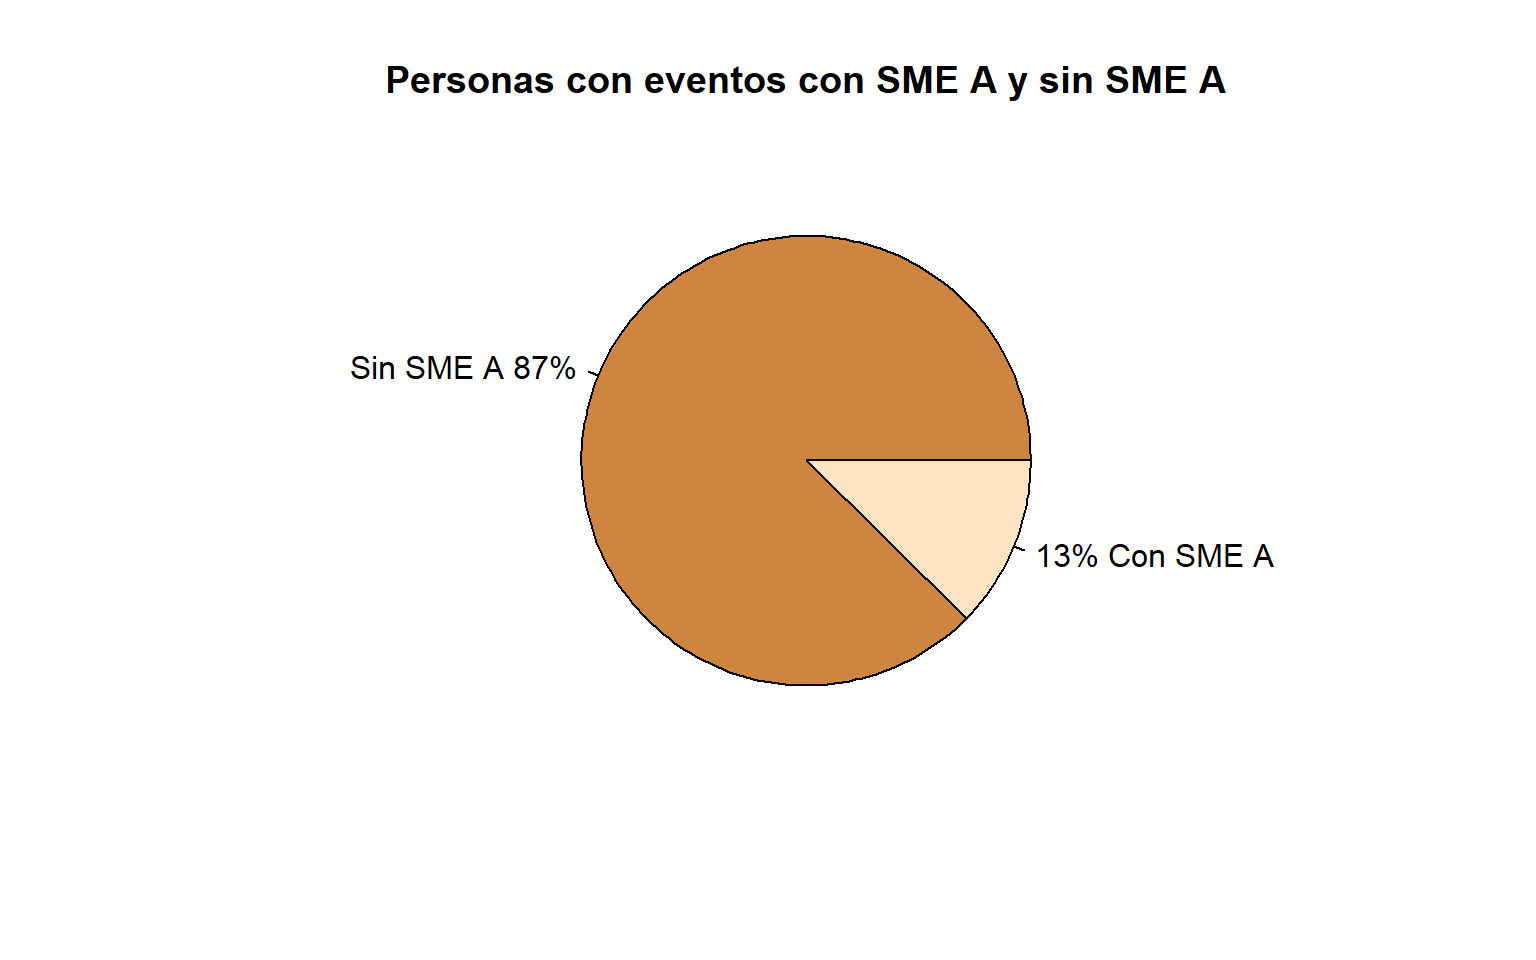
\includegraphics{index_files/figure-latex/persona con SMA-1.pdf}

\hypertarget{eventos-coronarios-segun-edad-y-genero}{%
\subsection{Eventos Coronarios Segun Edad y
Genero}\label{eventos-coronarios-segun-edad-y-genero}}

Al interpretar los gráficos se puede ver que los hombres tienen un pico
estable dentro de los 30 y 40 años, mientras que las mujeres presentan
un pico más pronunciado de eventos dentro del mismo rango de edad. Con
los datos de la tabla analizamos que 4 de cada 5 pacientes que ingresan
al hospital con eventos coronarios son hombres.

\begin{longtable}[]{@{}lll@{}}
\toprule
& Hombres & Mujeres\tabularnewline
\midrule
\endhead
Número de pacientes con eventos & 97 & 24\tabularnewline
Pico máximo de edad & 87 & 80\tabularnewline
\bottomrule
\end{longtable}

\hypertarget{pacientes-masculinos-que-presentan-eventos}{%
\subsubsection{Pacientes masculinos que presentan
eventos}\label{pacientes-masculinos-que-presentan-eventos}}

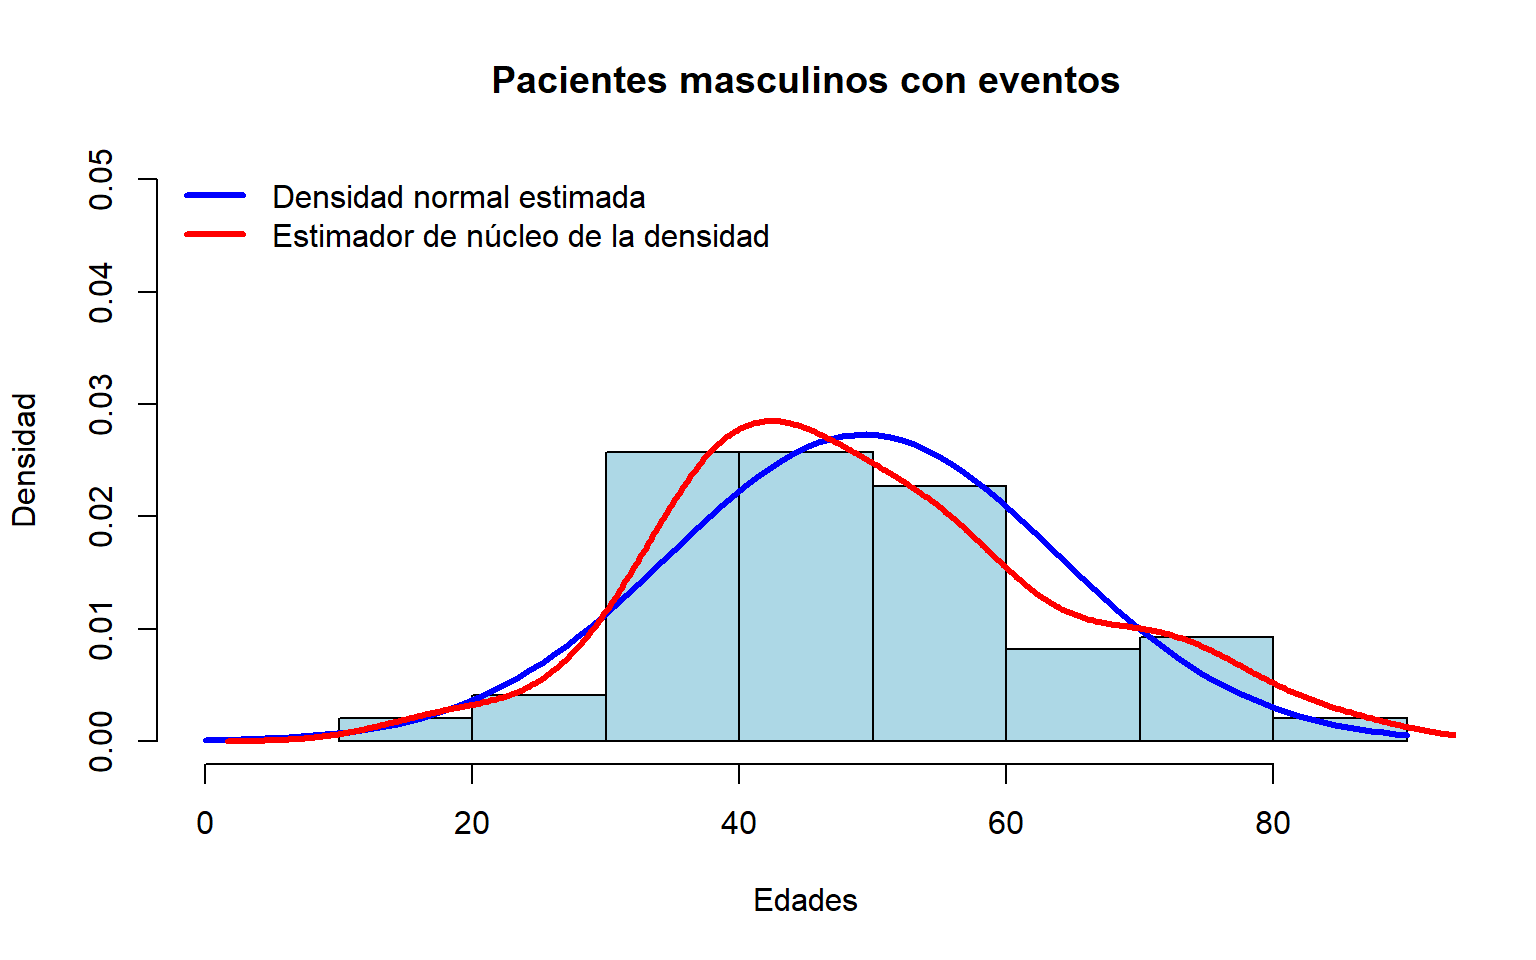
\includegraphics{index_files/figure-latex/eventos mas-1.pdf}

\hypertarget{pacientes-femeninos-que-presentan-eventos}{%
\subsubsection{Pacientes femeninos que presentan
eventos}\label{pacientes-femeninos-que-presentan-eventos}}

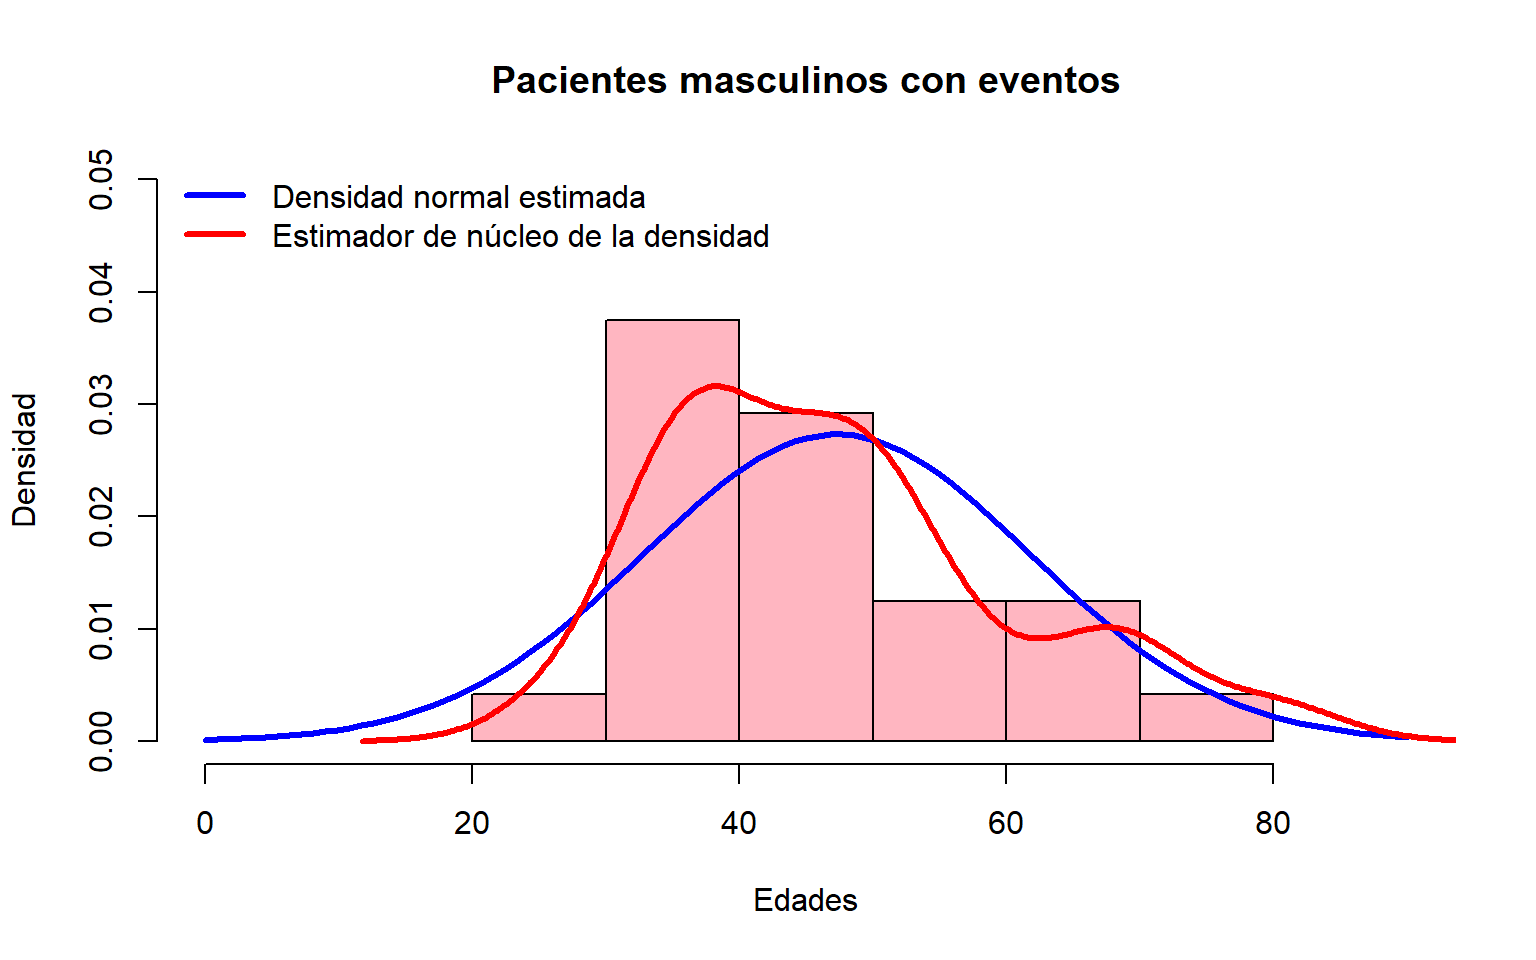
\includegraphics{index_files/figure-latex/eventos fem-1.pdf}

\hypertarget{los-diabuxe9ticos-los-obesos-y-la-hipertensiuxf3n-arterial}{%
\subsection{Los Diabéticos, los Obesos y la Hipertensión
Arterial}\label{los-diabuxe9ticos-los-obesos-y-la-hipertensiuxf3n-arterial}}

\hypertarget{diabuxe9ticos-obesos}{%
\subsubsection{Diabéticos obesos}\label{diabuxe9ticos-obesos}}

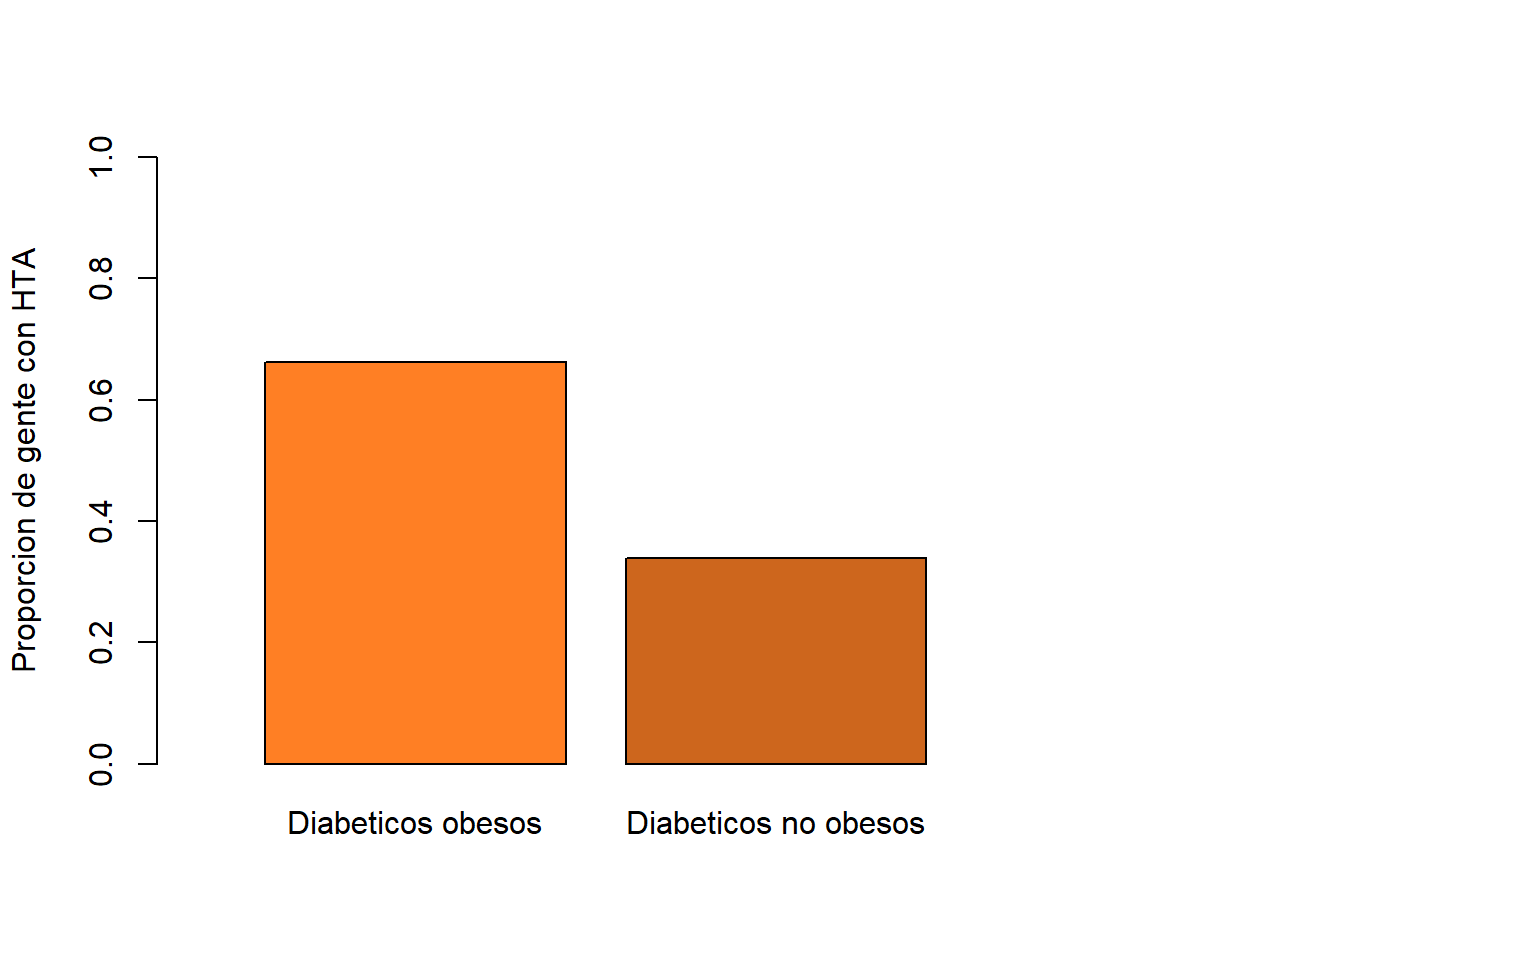
\includegraphics{index_files/figure-latex/diabeticos-1.pdf}

Buscamos la relación entra la obesidad y la tendencia a tener diabetes.
Y como a su vez ese grupo de personas tiene a tener HTA

\hypertarget{diabeticos-con-hta}{%
\subsubsection{Diabeticos con HTA}\label{diabeticos-con-hta}}

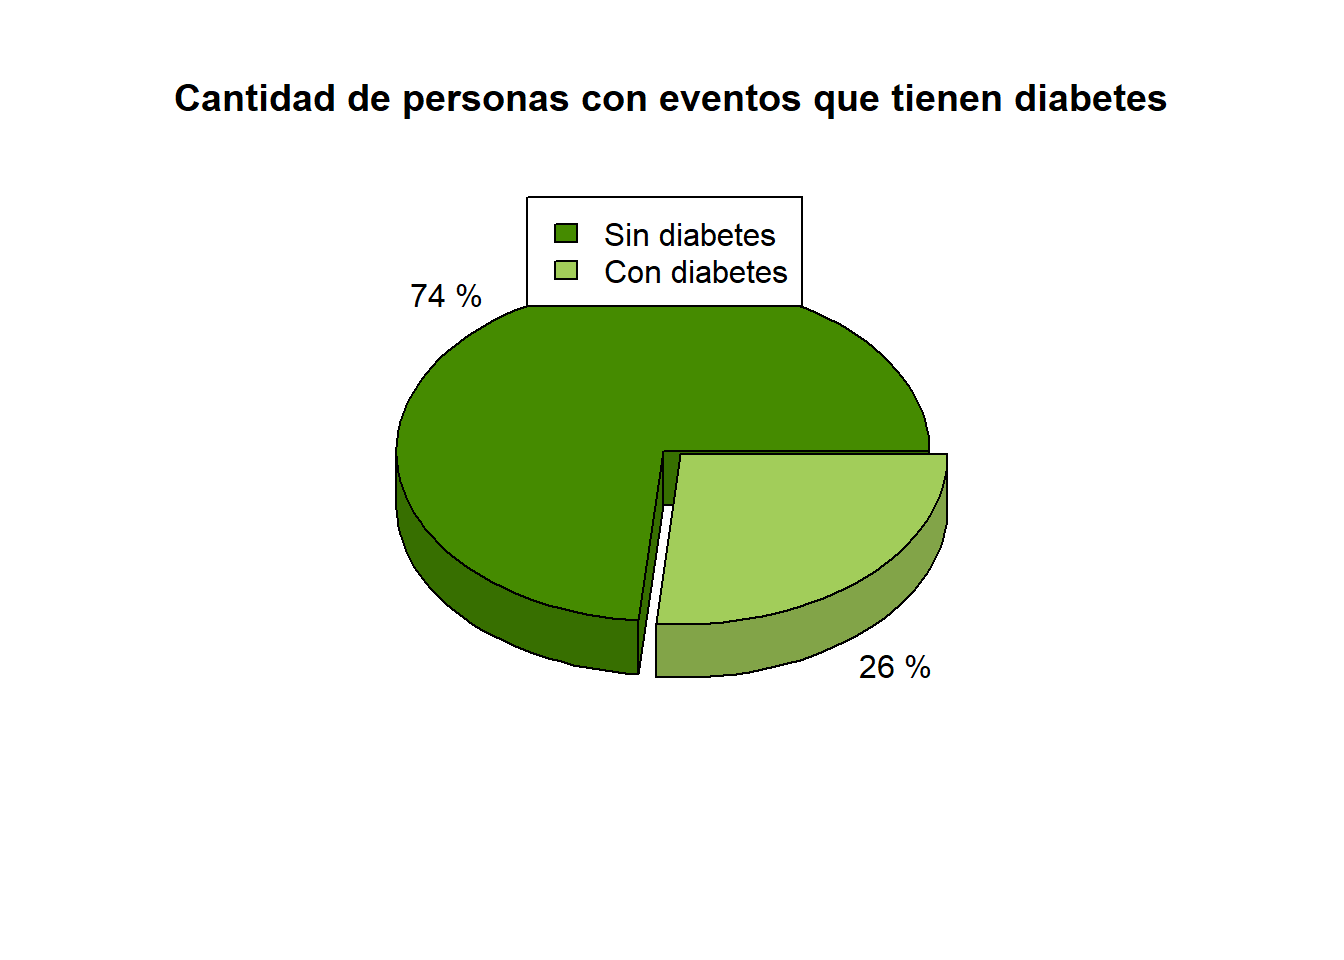
\includegraphics{index_files/figure-latex/cars-1.pdf}

Teniendo en cuenta los datos anteriores comparamos la tendencia de la
diabetes a los eventos cardiacos.

\hypertarget{relaciuxf3n-entre-fumadores-y-obesos}{%
\subsection{Relación entre Fumadores y
Obesos}\label{relaciuxf3n-entre-fumadores-y-obesos}}

Se analizó la relación de los pacientes que tienen obesidad y que son
fumadores, en cuanto a la tendencia de tener eventos cardiacos. La base
de datos de pacientes no define si son fumadores activos o pasivos, por
lo cual se agruparon ambos.

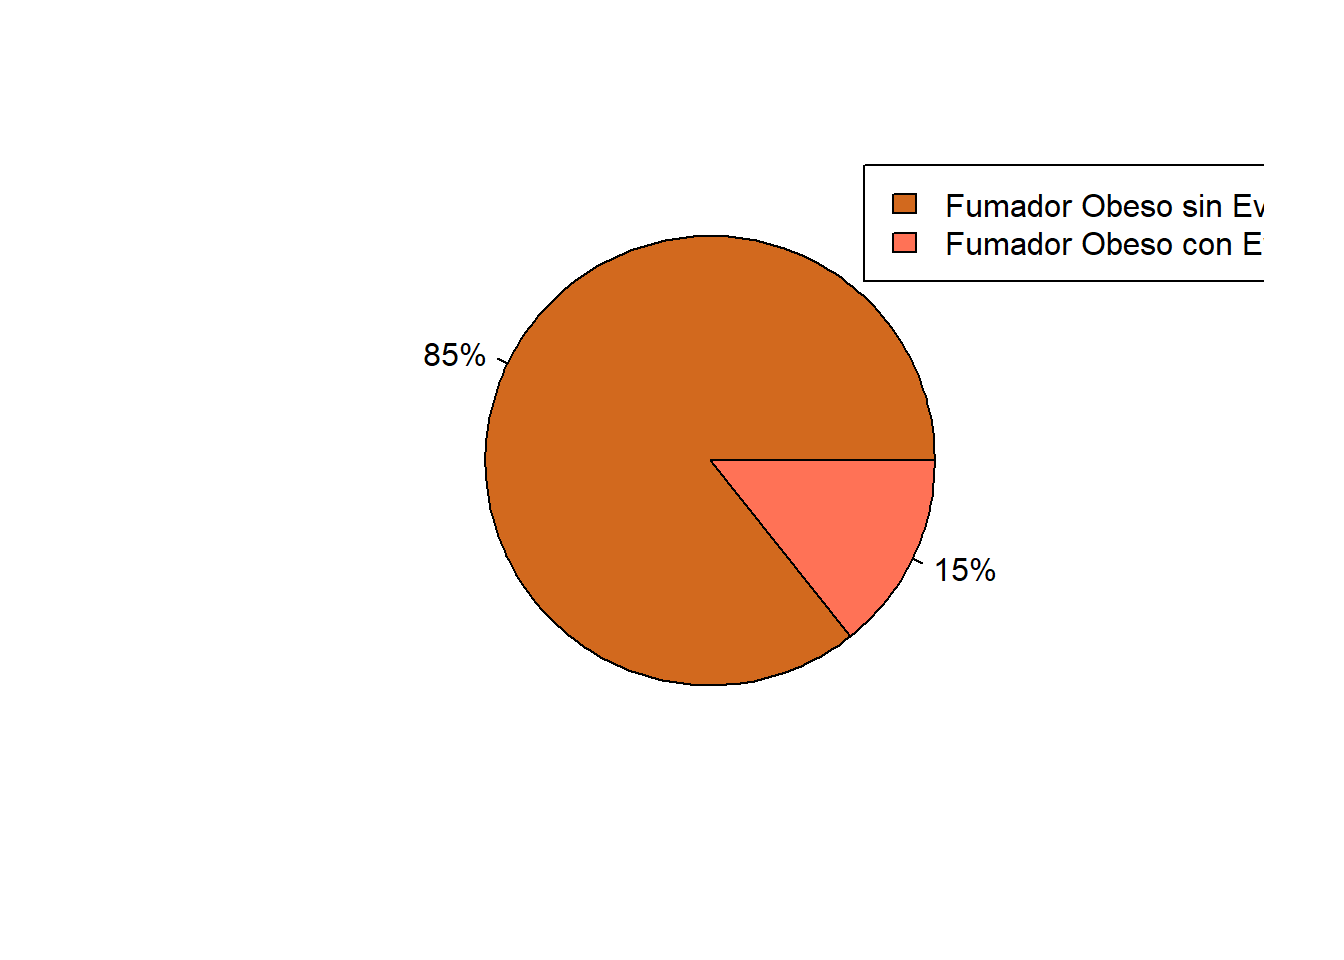
\includegraphics{index_files/figure-latex/Grafico Comparando Gente Adicta-1.pdf}
Dentro de la base de datos pudimos ver que el 10\% de los encuestados
tienen alguno de estos dos factores de riesgo. Del total de 121 personas
con eventos coronarios, 18 de estos son fumadores obesos, mostrando
cierta tendencia de estos dos factores.

\end{document}
